\section{Rakenne} \label{rakenne}
Seuraavaksi käydään läpi reunan rakennetta. Koska aihepiirinä on arkkitehtuurit, varsinaisten toteutettujen reunajärjestelmien rakennetta voidaan käydä ainoastaan hypoteettisesti. 
Eli mitä arkkitehtuuri mahdollistaa tai rajoittaa.
Ensimmäiseksi käsitellään reuna-arkkitehtuurien vaikutuksen toteutettavaan järjestelmään.
Tämän jälkeen esitellään reunan fyysisen rakenteen eri mallit, jossa keskeisessä osassa ovat reunasolmujen sijainnit.
Lopuksi käydään läpi reunan rakenteen merkitystä järjestelmän toiminnalle.



\subsection{Rakennetyypit}
Tässä kappaleessa käsitellään reunasolmujen muodostaman järjestelmän rakennetta. Rakenteet jakautuvat kahteen päätyyppiin: litteään ja hierarkiseen.
Litteä rakenne edustaa perinteisempää lähestymistapaa reunasolmujen asetteluun. Hierarkinen rakenne puolestaan uudempaa ajatusmallia, jossa reunasolmut delegoivat tehtäviä suhteessa tehokkaammille reunasolmuille. 

Reunan rakenteeseen vaikuttaa useampi tekijä. Myöhemmässä kappaleessa \ref{cloudlet} käsiteltävien cloudlettien yhteydessä visioitu operaattoreista riippumattomat reunasolmut mahdollistaisivat esimerkiksi kauppakeskuksien ja yksityishenkilöiden hankkia omat reunalaskentaa suorittavat yksiköt. Tällaisessa tilanteessa keskeiseksi kysymykseksi nouseekin reunapalveluiden tuottamiseen käytettävä liiketoimintamalli. Yksinkertaisuuden vuoksi tässä kappaleessa aihetta käsitellään, kuin reunan rakenne olisi yhden entiteetin, esimerkiksi operaattorin, käsissä. 

\paragraph*{Reunavyöhyke}
Reunavyöhyke on tämän tutkielman puitteissa määritelty termi, jolla viitataan vyöhykkeeseen jolla reunasolmut sijaitsevat. Reunavyöhyke voi olla kapea tai leveä, jotka vastaavat suurinpiirtein seuraavaksi määriteltävää litteää ja hierarkista rakennetta. Kapea vyöhyke tarkoittaa että reunasolmut sijaitevat verkossa samalla tasolla. Leveä vyöhyke puolestaan viittaa tilaan jossa reunasolmujen etäisyys vaihtelee merkittävästi, esimerkiksi lähimmillä tukiasemassa ja kauimmillaan mobiiliverkon ulkopuolella sijaitsevassa palvelinsalissa.

\begin{figure}[tb]
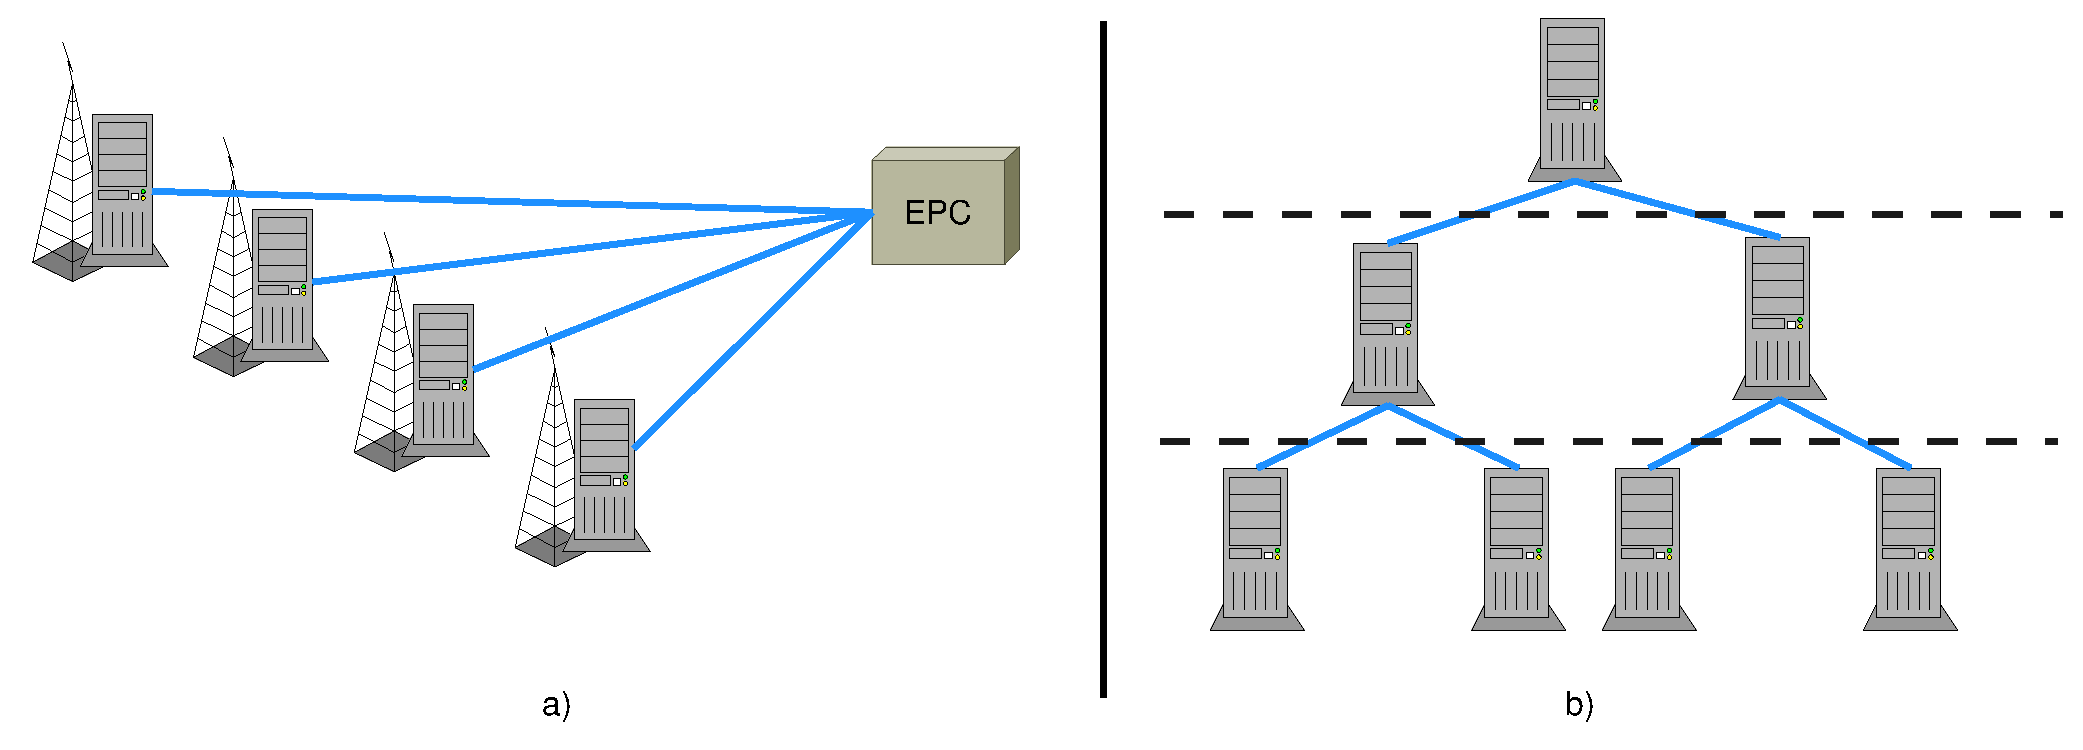
\includegraphics[width = \textwidth]{rakenne.eps}
\caption{Esimerkki rakenteet a) litteä rakenne b) hierarkinen rakenne kolmella tasolla} \label{fig:rakenne}
\end{figure}

\subsubsection{Litteä rakenne}
Litteällä rakenteella tarkoitetaan että jokainen reunasolmu on hierarkisesti samalla tasolla. Litteän järjestelmän keskeisin päätös on valita taso, jolle reunasolmut sijoitetaan. 

Yksinkertainen esimerkki tällaisesta toteutuksesta olisi reunajärjestelmä, jossa reunasolmut sijoitettaisiin mobiiliverkon tukiasemien yhteyteen kuten kuvassa \ref{fig:rakenne} a). Esimerkin järjestelmä  toteuttaisi äärimmäistä hajautusta ja lisäksi se olisi fyysisesti erittäin lähellä asiakaslaitetta. Tällaisessa rakenteessa on kuitenkin ilmeisiä ongelmia. Järjestelmän käyttö olisi teoriassa mahdollista ainaostaan niiden tukiasemien ympäristössä, joissa reunajärjestelmä sijaitsee. Tämän seurauksena reunalaskennan laajamittainen käyttöönotto olisi riippuvainen tukiasemiin sijoitettavien reunasolmujen hankinnasta. Mikäli oletetaan että siellä missä laskennan tarve on suurin, on myös eniten ihmisiä. Tästä yleensä seuraa että tällaisessa tilanteessa lähelle tuotu reunalaskenta on kalliimpaa, jo käytettävien tilojen hintojen vuoksi \cite{mao17}.

Vaihtoehtoinen ratkaisu olisi siirtää reunasolmuja kauemmaksi tukiasemista. Esimerkiksi siten että yksi reunasolmu vastaisikin useamman tukiaseman kautta tulevasta reunalaskennasta. Mobiiliverkko kontekstissa, reunasolmu sijaitsisi siis joko tukiasemien ja EPC:n välillä tai vasta EPC:n takana.  
Useamman tukiaseman niputtamista yhden reunasolmun vastuulle kutsutaan klusteroinniksi. 
Keskeisenä haasteena klusteroinnissa on valita oikean kokoiset klusterit ja sijoittaa oikea määrä resursseja kuhunkin klusteriin \cite{malandrino2016close}.
Klusterin suuruus ja viive todennäköisesti korreloivat jolloin on varottava tekemästä klustereista tarpeettoman suuria.
Reunasolmujen siirtäminen kauemmaksi asiakaslaitteista pitäisi siis mahdollistaa helpompi ja edullisempi käyttöönotto, koska tarvitaan suhteessa vähemmän reunasolmuja ja reunasolmujen ylläpito on näin ollen edullisempaa.
Kompromissina on kuitenkin suurempi viive reunasolmujen ja asiakaslaitteiden välillä. 
Onkin siis tärkeää että reunasolmuja ei viedä liian kauas reunasta, jolloin palvelun laatu heikkenee \cite{mao17}. 


Kuitenkin riippumatta litteän rakenteen sijainnista, sen pohjimmaisena ongelmana on resurssien kiinteys. Ympäristössä jossa reunalaskennan määrä vaihtelee, seuraa tilanne jossa reunasolmu on joko ylikuormitettuna tai alikuormitettuna suhteessa käytössä oleviin resursseihin \cite{tong2016hierarchical}. Jotta reunasolmut pystyisivät suoriutumaan kaikesta reunalaskennasta, reunasolmujen resurssit jouduttaisiin mitoittamaan rasitus-huippujen mukaan. Tästä seuraa lähes jatkuvaa alikuormitusta, joka tarkoittaa että reunajärjestelmän kustannukset olisivat korkeammat kuin olisi tarpeen. 
Tämän ongleman ratkaisuksi on esitetty hierarkista järjestelmää.


%In 2012, Flavio Bonomi and his colleagues introduced the term fog computing to refer to this dispersed cloud infrastructure. F. Bonomi et al., “Fog Computing and Its Role in the Internet of Things,”Proc. 1st Edition MCC Workshop Mobile Cloud Computing (MCC 12)


\subsubsection{Hierarkinen rakenne}
Hierarkinen rakenne on parannusehdostus reunalaskennan oletetulle litteälle rakenteelle \cite{tong2016hierarchical}
Reunasolmujen hierarkisella asettelulla tarkoitetaan järjestelmää, jossa reunasolmut on jaettu kerroksiin. Alimmalla kerroksella sijaitsevat reunasolmut ovat lähimpänä asiakaslaitetta, mutta niiden sisältämät laskentaresurssit ovat vähäisiä. 
Ideana on että alemmalla kerroksessa sijaitsevat reunasolmut voivat siirtää laskentaa ylemmällä kerroksella sijaitsevalle reunasolmulle, jolla on enemmän resursseja. Tasojen määrälle ei ole mitään rajaa, mutta useimmat ehdotukset sisältävät kaksi tai kolme tasoa. Kuvassa \ref{fig:rakenne} b) esimerkki kolmetasoisesta hierarkiasta.
Ylemmällä tasolla sijaitsevalla reunasolmulla on vastuullaan useampi alemman tason reunasolmu. Hierarkinen rakenne on siis puun mallinen.

Hierarkisen rakenteen keskeisenä tavoitteena on reunajärjestelmän resurssien käyttöasteen parantaminen \cite{tong2016hierarchical}. Ylemmillä kerroksilla sijaitsevat resurssit ovat suuremman joukon käytössä, hieman kuten litteässä mallissa tukiasemia klusteroitaessa. 
Hierarkisessa rakenteessa on kuitenkin riskinsä. Järjestelmän voidaan olettaa monimutkaistuvan jos laskentaa tehdään useassa kerroksessa. Ja etenkin järjestelmän ylempien kerroksien etäisyys asiakaslaitteisiin kasvaa, joka voi potentiaalisesti johtaa viiveiden kasvuun ja palvelun laadun heikkenemiseen.

Tong et al \cite{tong2016hierarchical} esittävät tukimuksessaan vertailua litteälle ja erilaisille hierarkisille rakenteille. Tilanteessa jossa järjestelmään on jaettavissa kiinteä määrä resursseja, kolmeen kerrokseen jaettu järjestelmä vaikutti optimaalisimmalta.
Vertailun mittarina käytettiin aikaa joka reunapalvelulla kului vastata annettuihin laskennallisiin tehtäviin. Kolmikerrokisen mallin etuina oli laskentaresurssien määrä ylemmillä kerroksilla. Tällöin etenkin ruuhkaisissa tilanteissa se suoriutui tehtävistään nopeammin kuin litteä. Lisäksi tutkimuksessa todettiin, että ylemmillä tasoilla sijaitseva tehokkaampi laskenta pystyy kompensoimaan siirtämisestä aiheutuvaa viivettä. Huomattakoon kuitenkin että tutkimuksessa käytettävä kuorma oli tyypiltään hienojakoista ja pientä. 


\subsubsection{Yhteenveto}
Hierarkinen järjestelmä on potentiaalinen vaihtoehto litteälle rakenteelle. Koska reunalaskennalle on monia hyvin erilaisia sovelluskohteita, hierarkinen rakenne vaatii tarkempaa tutkimusta erilaisilla reunalaskennan tyypeillä. Litteän rakenteen heikkoina puolina voidaan pitää sen kyvyttömyyttä sopeutua kuorman epätasaisuuseen, sekä järjestelmän ylläpidon kustannuksia, mikäli järjestelmää päätetään hajauttaa aggressiivisesti. Litteä järjestelmä on rakenteeltaan yksinkertainen ja se tukee esimerkiksi olemassa olevaa mobiiliverkon tukiasemien rakennetta. 


\subsection{Arkkitehtuurin vaikutus}
Edellisessä kappaleessa järjestelmän rakenteen oletettiin olevan vapaa sijoittamaan reunasolmut haluamiinsa paikkoihin. 
Todellisuudessa reuna-arkkitehtuurit kuitenkin asettavat joitakin rajoitteita reunsolmujen sijaintien suhteen. Seuraavaksi käsittelemme reuna-arkkitehtuurin vaikutusta reunasolmujen sijoitteluun.

%mobiiliverkko
Koska mobiiliverkko on usein asiakaslaitetta lähimpänä sijaitseva verkko, reuna-arkkitehtuurit ovat pyrkineet muodostamaan integraation sen kanssa.
Mobiiliverkon ja reunajärjestelmän integraatioissa voidaan puhua integraation sitovuudesta. 
Tällä tarkoitetaan kuinka sidoksissa reunajärjestelmä on mobiiliverkon rakenteeseen.
Monet ehdotetuista reuna-arkkitehtuureista ovat pyrkineet pitämään sidonnaisuutta mahdollisimman vähäisenä, jotta reunajärjestelmän käyttöönotto ei vaatisi mobiiliverkon uusimista.
Mutta mobiiliverkosta saatava tieto esimerkiksi tukiasemien handoverit ovat reunajärjestelmän kannalta oleellista tietoa, kun päätetään asiakaslaitteen laskennan suorittavasta reunasolmusta.
Tämä tarkoittaa siis että on lähes pakollista sijoittaa hallinnollisia toimia mobiiliverkon yhteyteen.
Vaikka reunan hallinnolliset toimet olisivat sidottuina mobiiliverkkon, reunasolmujen sijoitteluun on yleensä enemmän vapauksia. Etenkin tilanteessa jossa reunasolmulla ei itsellään ole hallinnollisia tehtäviä.
Ehdotettujen reuna-arkkitehtuurien keskuudessa on huomattavia eroja reunasolmunen mahdollisten sijaintien suhteen. Näitä käydään tarkemmin läpi luvussa \ref{ratkaisut}, jossa jokaisen arkkitehtuuriehdotuksen toiminnallisuus esitellään. 

Reuna-arkkitehtuurin riippuvuutta ympäröiviin järjestelmiin voidaan yrittää pienentää esimerkiksi ottamalla käyttöön SDN. SDN mahdollistaa tietoliikennevirtojen ohjaamisen siten että reunajärjestelmän tietoliikennevirrat eivät vaikuta mobiiliverkon toimintaan. Tämän seurauksena reunajärjestelmä on täysin vapaa sijoittamaan reunasolmut mobiiliverkon ulkopuolelle

Toinen ehdotettu ratkaisu on sitoa reunasolmut tukiasemiin. Tämä pakottaa järjestelmän reunasolmuille litteän rakenteen. Järjestelmä on siis reunasolmujen osalta sidoksissa mobiiliverkkoon. Small Cell Cloud (käsitellään kappaleessa \ref{scc}) käyttää tämänkaltaista ratkaisua. Ideana on että tukiasemat ovat tyypiltään \textit{pienisoluisia}, jolloin tukiaseman kantama olisi pieni ja täten palveltavien asiakaslaitteiden määrä myös vähäinen. Tämä mahdollistaisi reunalaskennan vaatimien laskentaresurssien sijoittaminen tukiaseman yhteyteen.

Kolmas ja viimeinen tyyppi on kokonaan mobiiliverkon ulkopuolelle sijoitettu reunajärjestelmä. Tämä antaa käytännössä täydellisen vapauden sijoitella reunasolmuja. Esimerkki tämänkaltaisesta järjestelmästä on Follow Me Cloud (käsitellään kappaleessa \ref{fmc}). Reunajärjestelmän sijoittaminen mobiiliverkon ulkopuolelle tarkoittaa että asiakaslaitteen ja reunasolmun välinen viive on vähintään se aika joka tietoliikenteellä kuluu mobiiliverkossa. Follow Me Cloudin tapauksessa oletetaankin että mobiiliverkon sisäistä viivettä voitaisiin minimoida ja että reunasolmut sijaitsisivat välittömästi mobiiliverkon ulkopuolella. 

%arkkitehtuurin asettamat rajoitteet
%hallinnon sijainti
%integraatio mobiiliverkkoon
%hallinnoivan järjestelmän omistajuus.

%mobiili














